\documentclass[11pt,a4paper]{scrartcl}

\parskip 0.5em plus 0.5em

\pagestyle{headings}

\usepackage{graphicx,hyperref}
\usepackage[tablegrid]{vhistory}

\date{\vhCurrentDate}
\author{\vhListAllAuthors}
\title{wiFred documentation -- Documentation for WiFi throttle with withrottle interface and wireless clock driver}

\begin{document}
\thispagestyle{empty}
\maketitle

\begin{abstract}

  This document describes the usage and configuration of the wiFred -- a very simple wireless throttle to connect to withrottle servers like JMRI -- and the wireless clock driver used to drive a simple wallclock to the timing of JMRIs FastClock system. It also contains schematics and BOMs for both devices as well as programming instructions and assembly tips, and also an overview of options for the server side of things.

The most recent version of this document can be found at:

\textit{https://github.com/newHeiko/wiFred/raw/master/documentation/docu.pdf} and

\textit{https://github.com/newHeiko/wiFred/blob/master/documentation/docu.tex}.

Skip right ahead to section~\ref{throttle} or~\ref{clock} if you are not interested in the why and more into the how.

\end{abstract}

\clearpage

\tableofcontents

\clearpage

\section{Background for wiFred development} \label{background}

As of the writing of this document, JMRI~\cite{jmri} has a long track record of offering a server for using smartphones as wireless model railroad throttles, along with apps like withrottle~\cite{withrottleApp}\footnote{withrottle is also the name JMRI uses for the protocol and the server.} and EngineDriver~\cite{EngineDriver}. This server will enable WiFi throttles to control locos any model railroading layout to which JMRI can build a connection~\cite{jmrihardwaresupport}. In addition, Digitrax~\cite{digitrax} and MRC~\cite{mrc} offer specific hardware solutions to enable the connection of the abovementioned smartphone apps to their DCC systems through a WiFi network.


The Fremo~\cite{fremo} is a European modular model railroading club whose unique requirements on it's DCC throttles led to the creation of the throttles FRED and FREDI~\cite{fred} -- a series of LocoNet\textregistered-throttles which started their life as hobbyist projects with large numbers in circulation but were also commercially available from Uhlenbrock~\cite{uhlenbrock}.

\subsection{Specification wishlist}

In modular railroading events, particularly of the Fremo-americaN-group~\cite{fremo}, some people have evaluated the smartphone throttle solutions and found them lacking a nice, haptical feedback. But the idea of wireless control without locking into a specific vendor and their necessarily expensive equipment found great approval. So a wishlist was compiled to define the requirements for a wireless throttle:
\begin{itemize}
\item Same form factor as the FRED~\cite{fred} with similar controls
\item Option to control at least two, better four locomotives for double/triple traction (similar to the double FRED)
\item Battery runtime of at least six hours
\item Exchangeable batteries, so when the battery runs down, they can be quickly exchanged for a charged set or cheap primary cells
\item Easy configuration, but not too easy to prevent operators from accidentally selecting other locomotives
\item As little change to the existing Fremo Loconet\textregistered\ network as possible
\item Use of withrottle protocol, so the server side of the communication can be assumed to work and does not have to be developed as well
\end{itemize}

\subsection{Wireless clock}

During the development of this wiFred another topic came up in the americaN group of the Fremo, namely wireless clocks with adjustable clock rate for Timetable \& Trainorder operations. Contrary to other Fremo groups, the americaN group standard does not call for any cabling for fast clocks and the group does not have the equipment for setting up a fast clock network, so first trails were done with regular Quartz clocks at 1:1 rate which had to be adjusted to timetable starting time every timetable morning. So a new solution was required, adding the following to the specification above:

\begin{itemize}
\item Battery runtime of at least eight hours to have some backup for long days
\item Able to control cheap Quartz clocks
\item Clock rate adjustable centrally in small increments in case the timetable planner has misjudged the capacity of the layout or operators
\item Re-use existing systems as much as possible -- in the case of the clock system, use JMRIs fast clock server
\end{itemize}

\clearpage

\section{wiFred Wireless throttle} \label{throttle}

\subsection{Quickstart Guide}

Follow these steps for a new throttle (see later chapters for more explanation or if you run into trouble)

\begin{enumerate}
  \setcounter{enumi}{-4}
\item Use PCB to determine positions of holes and cutouts in housing
\item Make said cutouts and glue little pieces of 3mm thick plastic or wood underneath PCB screw holes  
\item Solder components to PCB
\item Flash firmware to ESP and to AVR
\item Test fit PCB into housing, removing plastic parts of housing as required
\item Fit PCB into housing, insert three screws to fix PCB to housing
\item Make sure communication jumpers are set correctly, close housing and fix back cover with two screws
\item Add throttle knob
\item Insert batteries
\item Using any WiFi client (laptop, smartphone, tablet...), find and connect to network \textit{wiFred-configXXXX}
\item Using any web browser, navigate to \textit{http://192.168.4.1}
\item Enter your WiFi configuration (and a throttle ID if you like -- highly recommended to easier tell them apart) \textbf{and hit the \textit{Submit}-Button}
\item Click on \texttt{Loco configuration subpage}
\item \textbf{Make sure to enable the checkbox on top next to \texttt{Enabled?}} and also enter your wiThrottle server settings
\item For every loco you want to control with this throttle, enter the appropriate details below
\item Finish by \textbf{hitting the \textit{Submit}-Button}
\item Configure function settings for each loco on the respective sub pages if required
\item Restart the throttle by navigating back to the main configuration page and clicking on \texttt{Restart system to enable new WiFi settings}
\end{enumerate}

Your throttle should now be ready to use and connect to your wiThrottle server on startup. Refer to the chapters below if it does not or contact the author of this document.

\subsection{Usage}

\begin{figure}[tbh]
  
  \centering
  \includegraphics[height=100mm]{images/throttle_Front}
  \hspace{1em}
  \includegraphics[height=100mm]{images/throttle_Back}
  \hspace{1em}
  \includegraphics[height=100mm]{images/throttle_Back_openBattery}

  \caption{Controls and features of the wiFred-throttle}
  \label{throttleControls}

\end{figure}

Figure~\ref{throttleControls} shows the controls of the wireless throttle. They consist of the following:

\begin{itemize}
\item Four loco selection switches (loco 1 on the left, loco 4 on the right, move towards speed potentiometer to enable)
\item Speed potentiometer (Counter-clockwise endstop: Stop, clockwise endstop: Full speed)
\item Direction switch -- move right for forward movement, left for reverse movement
\item Black function keys F0 to F4
\item Two yellow shift keys to trigger F5-F8 (SHIFT1, lower key), F9-F12 (SHIFT2, upper key) and F13-F16 (both shift keys)
\item Red emergency stop key
\item Two green direction indicator LEDs
\item One red status LED
\item Battery compartment (on the rear) for two AA cells, 1.2\,V to 1.5\,V nominal voltage
\end{itemize}

As soon as a pair of batteries is inserted into the battery compartment as the symbols inside the battery compartment show, the throttle will boot up and try to connect to a wireless network. The throttle will not be damaged if batteries are inserted wrongly, but it will not work either. Use NiMH- or primary AA cells with 1.2\,V to 1.5\,V nominal voltage, low self discharge NiMH cells like Eneloop\textregistered\ or similar are recommended. Do not insert 3\,V or 3.6\,V AA size lithium batteries as this may damage the throttle.

If no connection to the network configured into the device can be established within 60 seconds, the throttle will create it's own wireless network named \textit{wiFred-config} plus four hex digits taken from the MAC address of the throttle WiFi interface, for example \textit{wiFred-config0CAC}, to enable configuration as described in the next section.

Four different locos with long DCC addresses can be assigned to the four loco selection switches. Commands derived from the speed potentiometer, the direction switch and the function keys will be transmitted to all selected locos (near) simultaneously, with a certain translation table enabling some locos to go backwards when others go forwards and also limiting function keys to some of the four locos only -- this is described in more detail in sections~\ref{throttle_LocoConf} and~\ref{throttle_FunctionConf}.

Pushing the red emergency stop key will cause the throttle to send an emergency stop signal to all four locos attached. After an emergency stop, turn the speed potentiometer to zero to re-enable control of the locos.

Pushing the red emergency stop key while holding down either of the shift keys will place the device into configuration mode (as well as issueing an emergency stop to all attached locos). See section~\ref{throttle_Conf} for more details on how to access the throttle to do the configuration.

Any change in the loco selection switches will cause the throttle to send a stop (zero speed) command to all attached locos. This makes sure that any loco that is deselected will stop on the layout and avoids newly selected locos suddenly taking off at speed. The same is true for a change in the direction switch, to avoid high-speed reverse maneuvers. Turn the speed potentiometer to zero to re-enable control of the locos.

When all four loco selection switches are set to the disabled state, the throttle will send a stop (zero speed) command to all four locos attached and -- after a wait time of 30 seconds -- it will disconnect from the network and go into low power mode. To reconnect, re-enable any loco selection switch.

The same happens when the batteries are empty, but the throttle will not reactivate before changing the batteries. Expected runtime with a pair of 2500\,mAh-NiMH-batteries is around 8-10 hours of full time operations, more if the throttle is placed in low power mode when the locos are not running.

During startup and operation, the LEDs will show the patterns explained in table~\ref{ledTable}.

\begin{table}
  \caption{LED patterns and their meaning on the wiFred throttle} \label{ledTable}

  \vspace{0.5em}

  \centering
  \begin{tabular}{| m{6em} | m{6em} | m{6em} | m{15em} |}
    \hline
    Red LED & Green LED (Left) & Green LED (Right) & Status \\
    \hline
    \hline
    Slow Blinking (0.5\,Hz) & Off & Off & Trying to connect to WiFi network \\
    \hline
    Fast Blinking (2\,Hz) & Off & Off & Successful WiFi connection, trying to connect to wiThrottle server and acquire locos \\
    \hline
    \hline
    Off & Off & On & Regular operation, forward direction \\
    \hline
    Off & On & Off & Regular operation, reverse direction \\
    \hline
    Off & Flashing & On & Emergency stop, forward direction. Also happens when switching direction with speed potentiometer not at zero \\
    \hline
    Off & On & Flashing & Emergency stop, reverse direction. Also happens when switching direction with speed potentiometer not at zero \\
    \hline
    \hline
    Off & Off & Blinking & Battery low, regular operation, forward direction \\
    \hline
    Off & Blinking & Off & Battery low, regular operation, reverse direction \\
    \hline
    Off & Flashing & Blinking & Battery low, Emergency stop, forward direction \\
    \hline
    Off & Blinking & Flashing & Battery low, Emergency stop, reverse direction \\
    \hline
    Short flashes & Off & Off & Throttle in low-power mode \\
    \hline
    Off & Off & Off & Battery empty or no battery inserted \\
    \hline
    \hline
    On & Off & Off & No connection to existing WiFi network. Created internal configuration WiFi network \\
    \hline
    On & On & On & Configuration mode enabled while connected to existing WiFi network. All locos emergency stop to avoid runaways. Push SHIFT + ESTOP again to exit configuration mode \\
    \hline
    
  \end{tabular}

  \vspace{0.5em}

  To recover from an emergency stop, turn speed potentiometer to zero to re-gain control.
  
\end{table}

\subsection{Configuration} \label{throttle_Conf}

Before using the device, it must be configured. At the very least, the General Configuration~\ref{throttle_GeneralConf} and Loco Configuration~\ref{throttle_LocoConf} pages have to be submitted once to be saved to non-volatile memory. If no valid configuration is detected at startup, the device will start with a default configuration with no locos enabled and trying to connect to a network named ``undef'' with a key named ``undef'', which will probably fail.

\subsubsection{Entering configuration mode}

There are two ways to enter configuration mode:

\begin{enumerate}
\item Power up the throttle when the configured WiFi network is not in range (or when there is no valid configuration -- the first startup of a new throttle will fall into this category)
\item Press SHIFT (either key) and ESTOP together when the throttle is connected
\end{enumerate}

In the first case, the throttle will create a wireless network named \textit{wiFred-config} plus four hex digits taken from the MAC address of the throttle WiFi interface, for example \textit{wiFred-config0CAC}. Any WiFi device with a web browser can connect to that network and open a web browser to point to \textit{http://192.168.4.1}.

In the second case, the throttle will change the last tuple of it's IP address to .253 -- so if the wireless network is configured with IP addresses in the \textit{192.168.100.x}-range as highlitghted in figure~\ref{withrottleScreenshot}, any web browser can access the configuration at \textit{http://192.168.100.253}.

If the IP address of the throttle during normal operation is known, the configuration page can also be accessed by pointing a web browser to it at any time while it is connected. Note that this is untested and therefore not recommended while the throttle is running locos.

\begin{figure}[tbh]
  \centering
  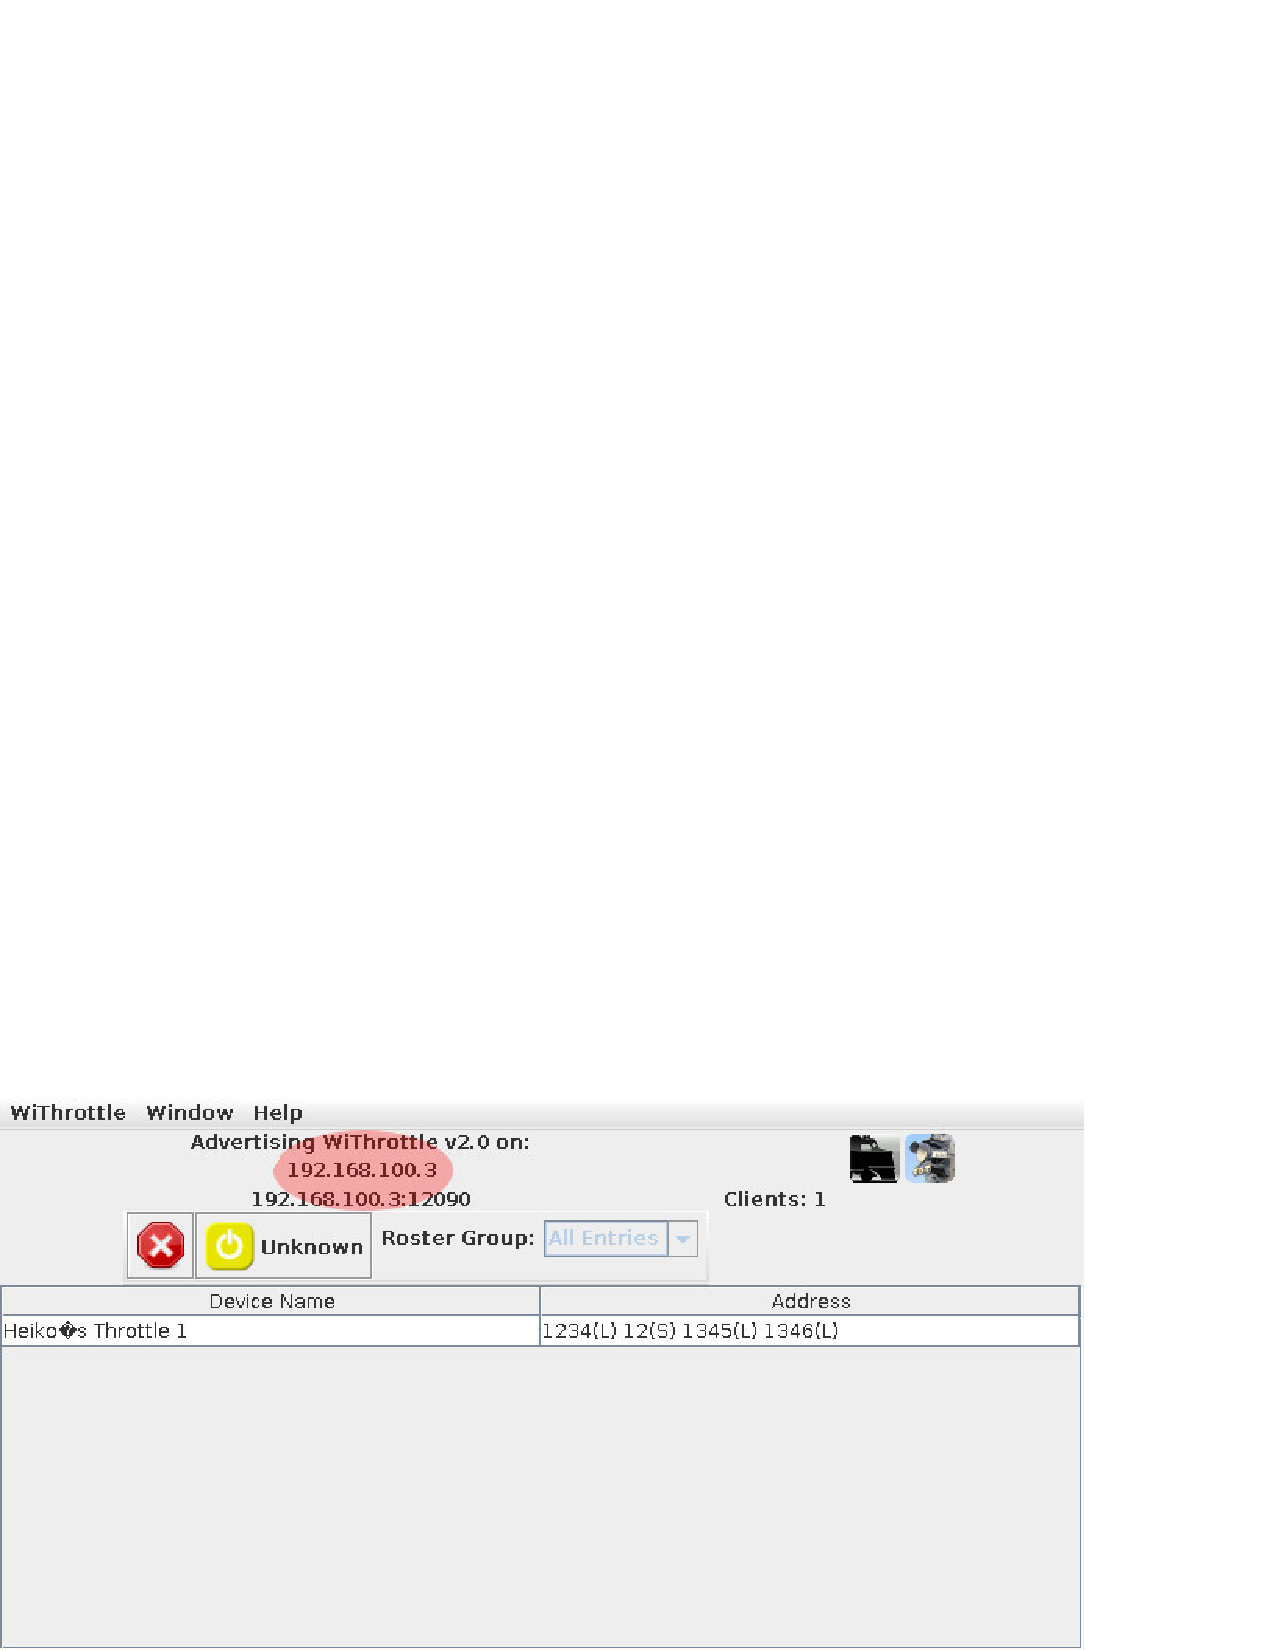
\includegraphics[width=0.8 \textwidth]{images/withrottle_Screenshot}
  \caption{Screenshot of wiThrottle screen showing one throttle connected}
  \label{withrottleScreenshot}
\end{figure}

\subsubsection{General configuration} \label{throttle_GeneralConf}

\begin{figure}[tbh]
  \centering
  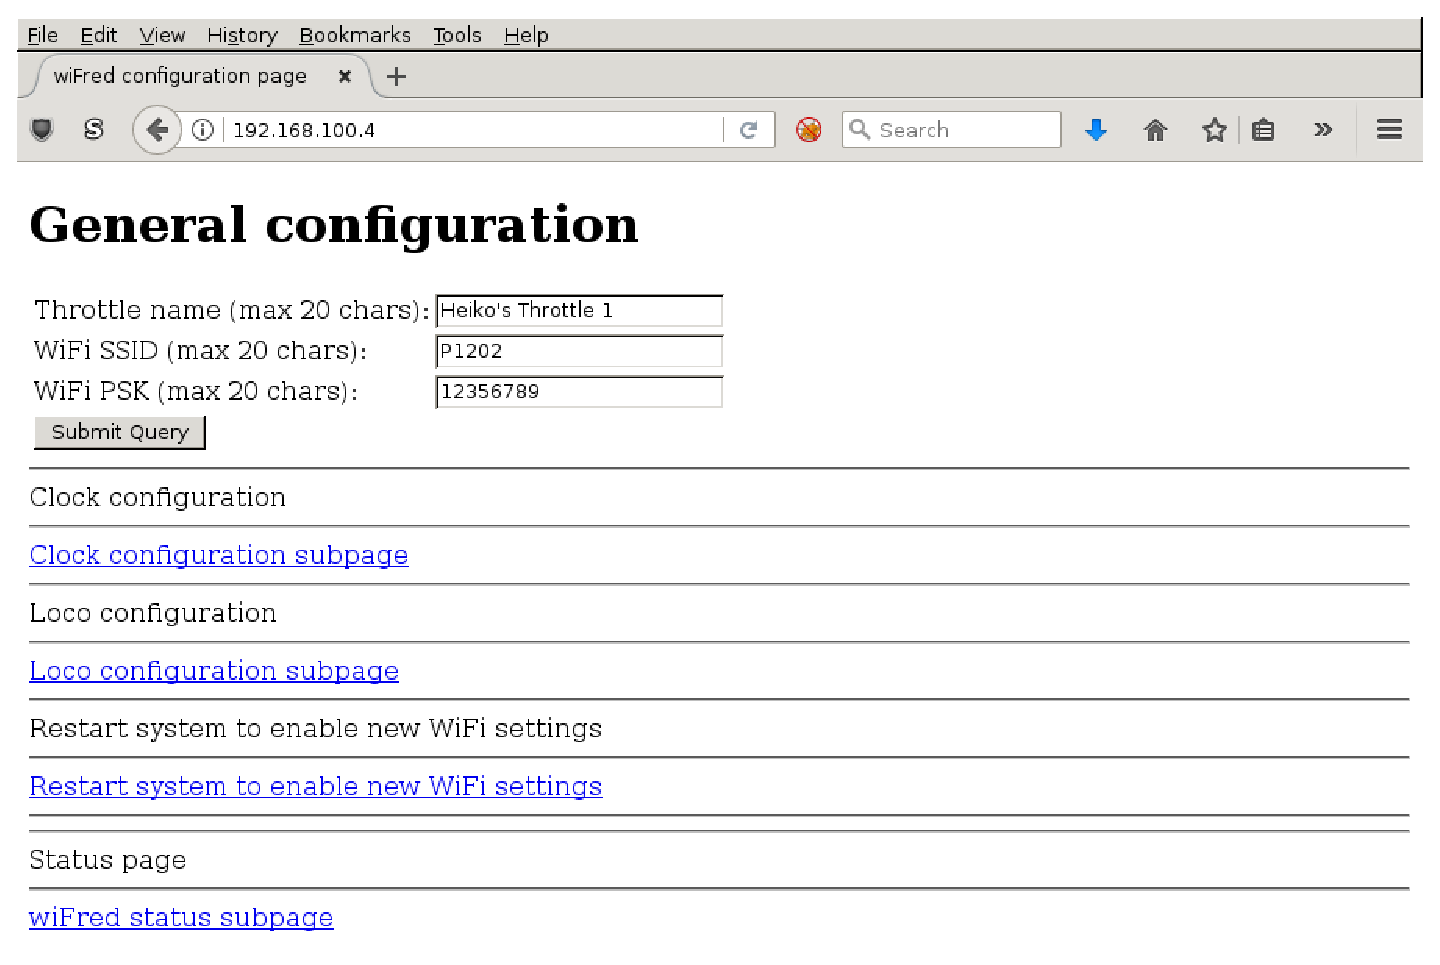
\includegraphics[width=0.8 \textwidth]{images/screenShot_main}
  \caption{Screenshot of wiFred main configuration page}
  \label{throttleConfMainPage}
\end{figure}

Figure~\ref{throttleConfMainPage} shows the first page you will see when you point a web browser at your wiFred throttle. It has some general configuration settings for the following items:

\begin{description}
\item{Throttle name:} This is a free-form identification string of the throttle. It shows up in the wiThrottle window of JMRI as shown in figure~\ref{withrottleScreenshot} and can be used to identify the throttle during configuration.
\item{WiFi SSID:} The name of the wireless network the throttle shall connect to.
\item{WiFi PSK:} The so-called password\footnote{Technically correct term: Pre-Shared Key} for the wireless network.  
\end{description}

\textbf{Reminder: Changes are saved using the ``Submit Query'' button which may look different in different web browsers (firefox shown).}

A new device will not read a saved configuration at startup unless both the main page and one of either the loco configuration subpage or the clock configuration subpage has been saved at least once.

\begin{figure}[tbh]
  \centering
  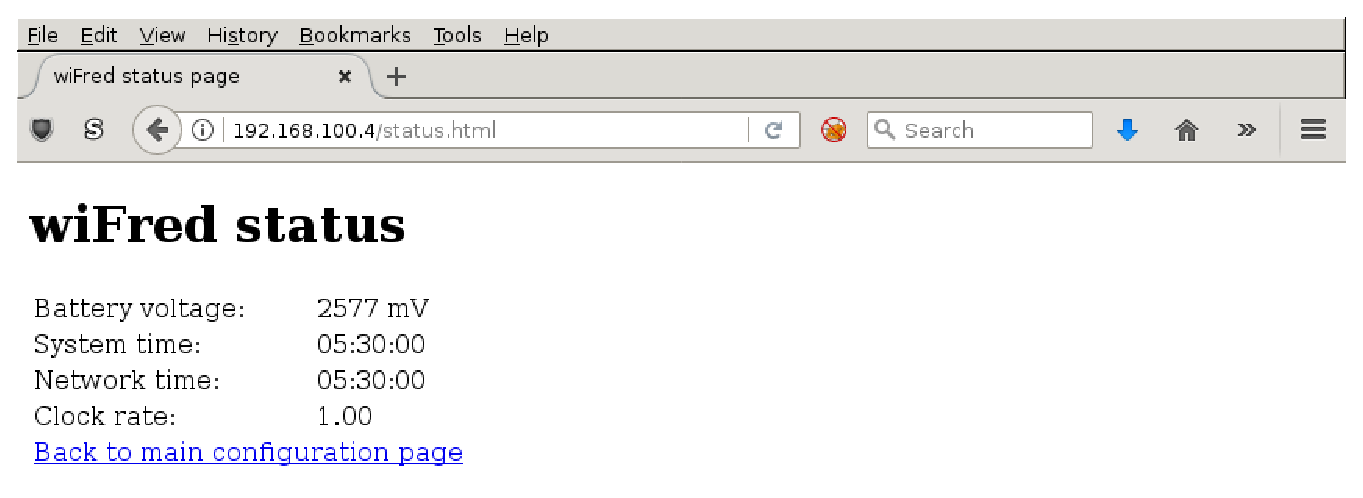
\includegraphics[width=0.8 \textwidth]{images/screenShot_status}
  \caption{Screenshot of wiFred status page}
  \label{throttleConfigStatusPage}
\end{figure}

This page also includes links to the configuration sub pages for locos and clock settings as well as a link to the status page shown in figure~\ref{throttleConfigStatusPage} which gives information about the current clock settings and battery voltage and may be enhanced in the future.

\subsubsection{Loco configuration} \label{throttle_LocoConf}

\begin{figure}[tbh]
  \centering
  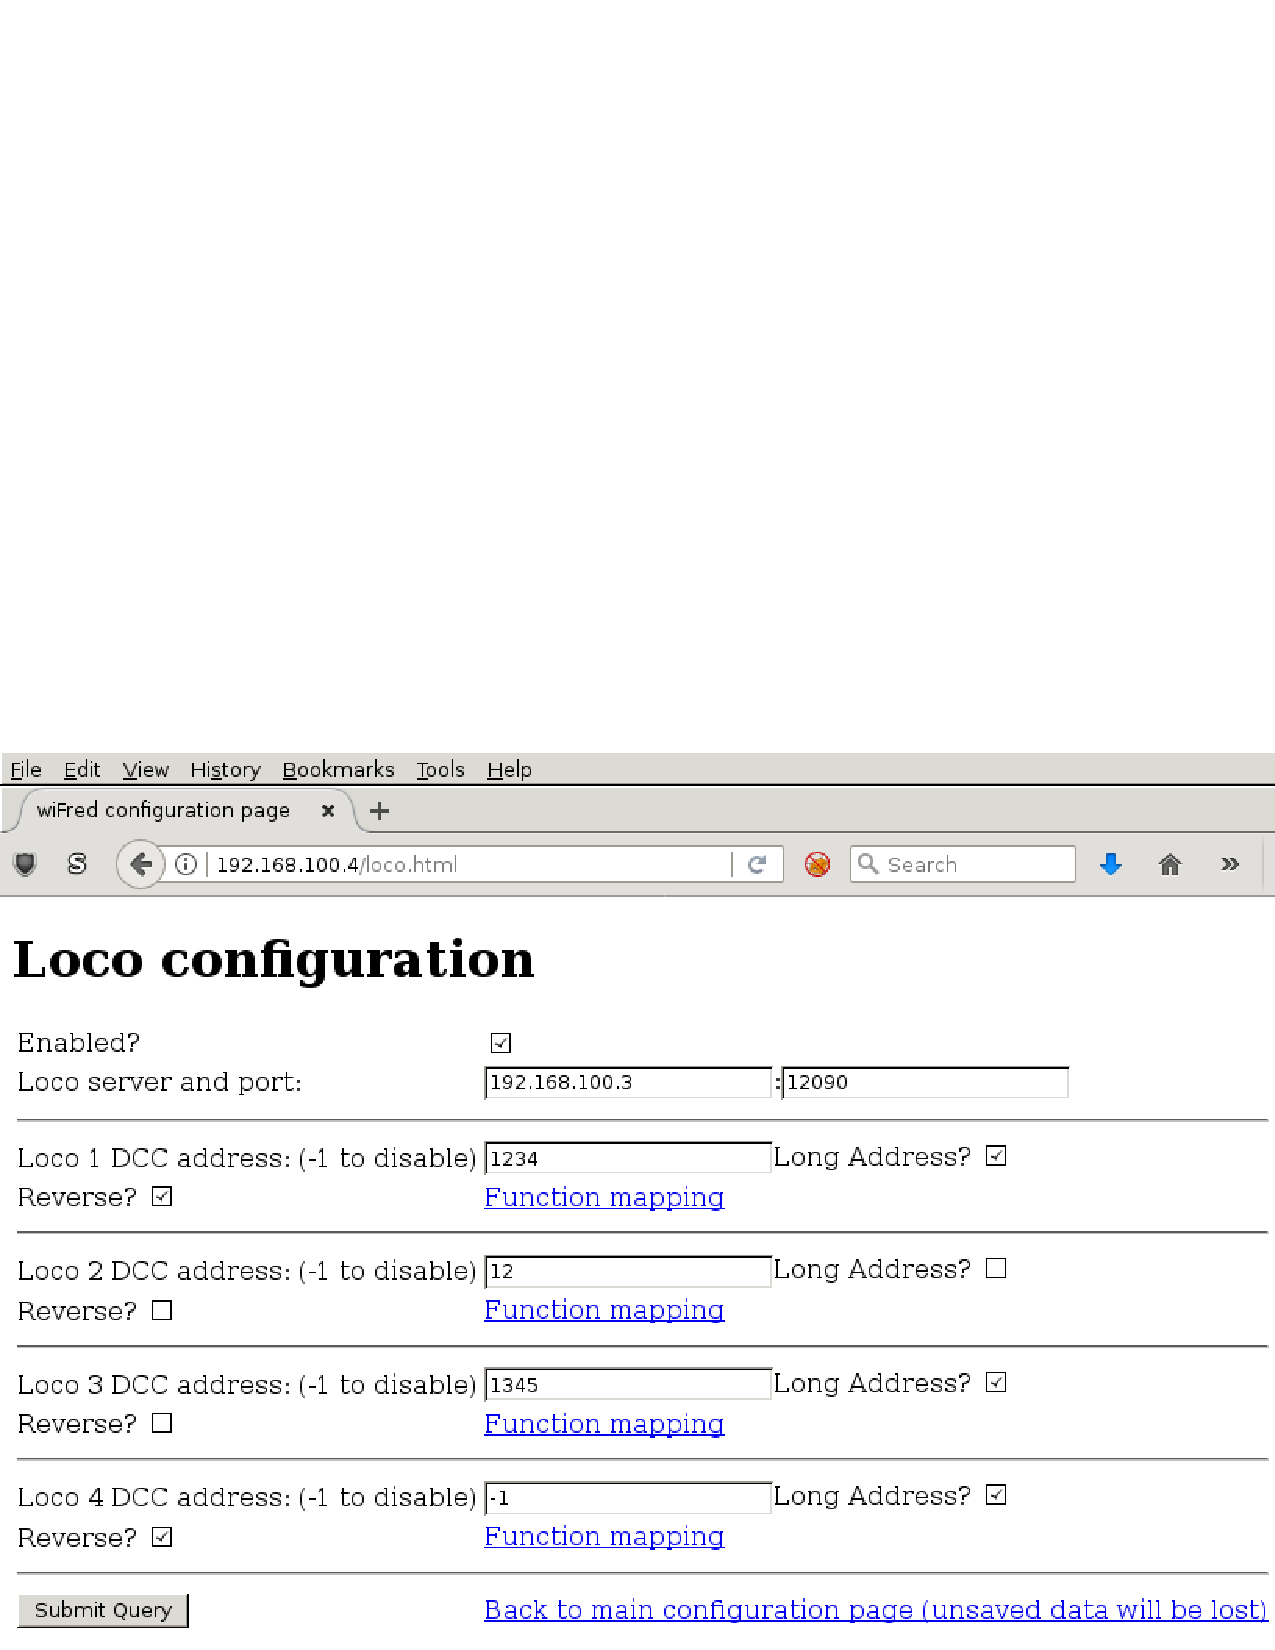
\includegraphics[width=0.8 \textwidth]{images/screenShot_loco}
  \caption{Screenshot of wiFred loco configuration page}
  \label{throttleConfigLocoPage}
\end{figure}

On this page, shown in figure~\ref{throttleConfigLocoPage}, the (up to four) locomotives to be controlled with this throttle and some settings for all locomotives are available.

Right on top, the checkbox next to \texttt{Enabled?} determines if the wiFred is to be used as a throttle. All the configuration settings are available if it is not, but it will not connect to the withrottle server and several other features described in this document may not work either unless this checkbox is enabled.

Next the server settings can be found. The correct settings can be read from the JMRI withrottle server screen, as highlighted in figure~\ref{withrottleScreenshot}. Normally the port does not need to be changed, as 12090 is the default setting.

Following the server configuration, there are four identical sections assigned to the four different locomotives which can be controlled with this throttle. Each section consists of the following settings:

\begin{description}
\item{DCC address:} Can be a short address between 1 and 127 (also used for consists) or a long address between 0 and 10239. Note: Short addresses between 1 and 127 are not the same as long addresses between 1 and 127. If this is set to -1, the corresponding loco is disabled.
\item{Long address?:} Checkbox to change the behaviour of the DCC address input field described above.
\item{Reverse?:} If checked, the corresponding loco will invert it's travel direction. Mainly intended for back-to-back consists without decoder reconfiguration.
\item{Function mapping:} Link to the function mapping subpage for the corresponding loco, as described in section~\ref{throttle_FunctionConf}. Clicking this link will lose all information entered on the current page and take the web browser to a different subpage.
\end{description}

\textbf{Reminder: Changes are saved using the ``Submit Query'' button which may look different in different web browsers (firefox shown).}

\subsubsection{DCC function configuration} \label{throttle_FunctionConf}

By default, if a function key is pressed, the throttle will send the appropriate commands to every loco under control. Under certain circumstances, this may not be desired -- the obvious example being a loco in the middle of a multi-unit consist, which should not have lights or ditchlights. So this page -- shown in figure~\ref{throttleConfigFunctionPage} -- offers the option to chose between three different settings for every function on each of the four locomotives (one page per locomotive):

\begin{figure}[tbh]
  \centering
  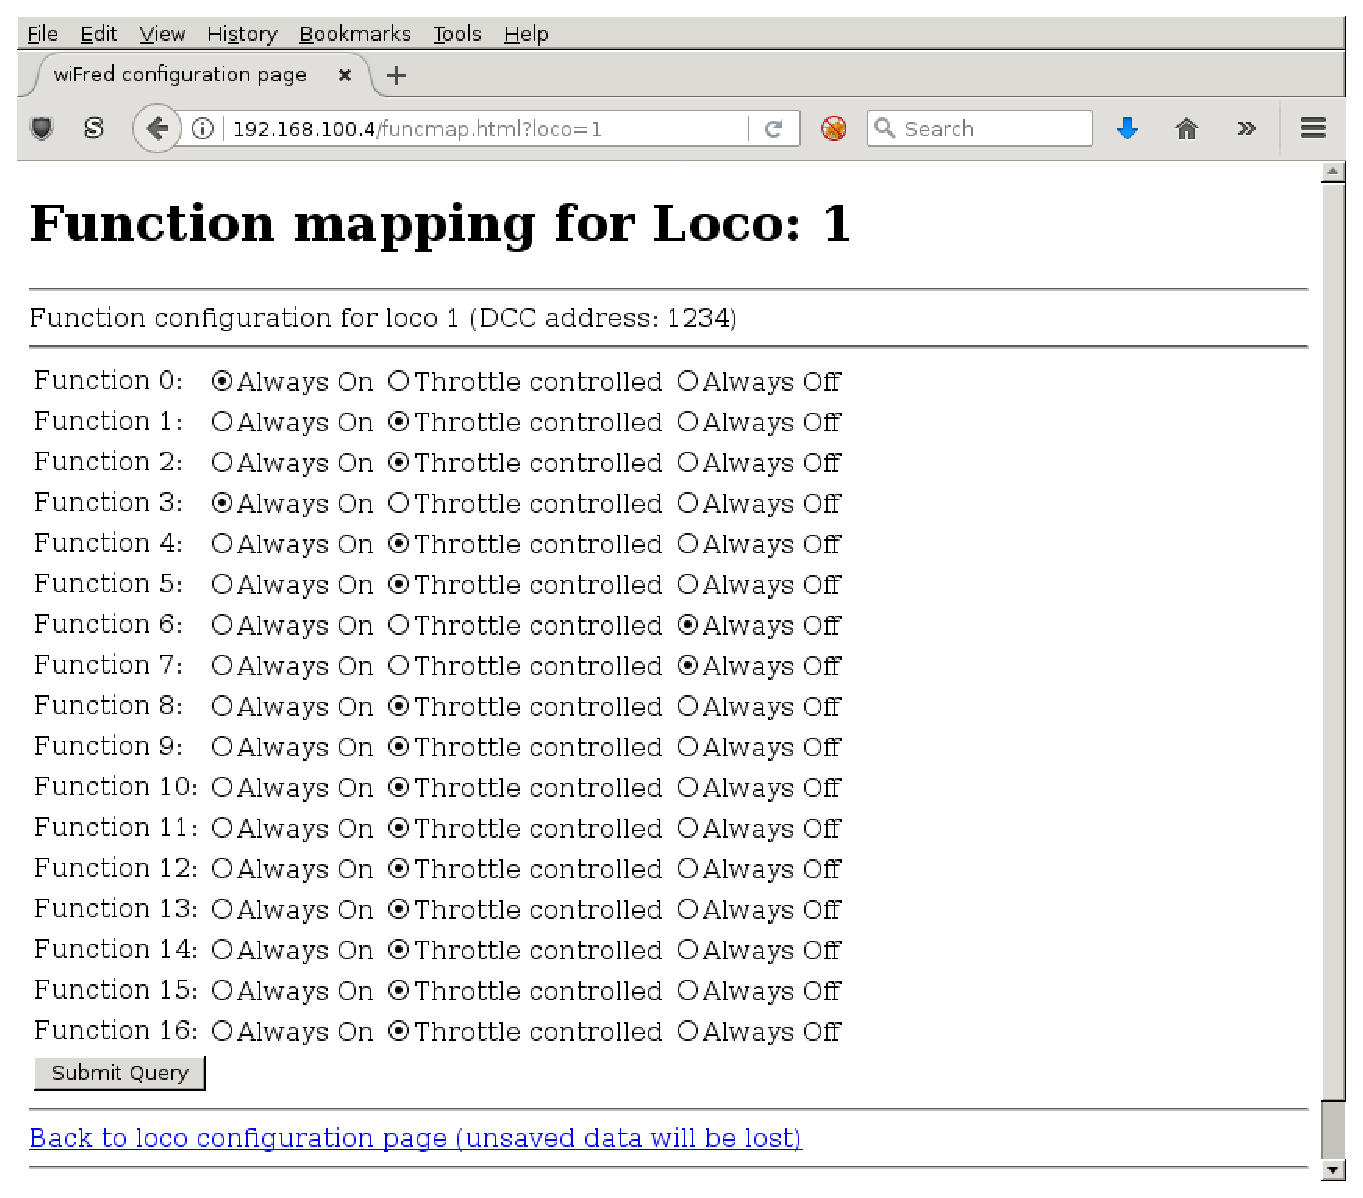
\includegraphics[width=0.8 \textwidth]{images/screenShot_functions}
  \caption{Screenshot of wiFred function handling config page}
  \label{throttleConfigFunctionPage}
\end{figure}

\begin{description}
\item{Always Off:} When the loco is enabled by moving the selection switch to the ``selected'' position, the current status of the function is queried. If the function is on, a function key press will be simulated to turn it off. No other function key events will be sent to this loco for this function.
\item{Throttle controlled:} When the first loco is enabled by moving the selection switch to the ``selected'' position, the current status of the function is queried and saved. When selecting the next loco, the status is queried. If it does not match the first loco, the function status is changed by simulating a function key press. Afterwards, key presses are handed through to the loco.
\item{Always On:} Similar to the ``Always Off'' setting, but the throttle will attempt to enable the function when the locomotive is selected and ignore any further function key presses. This will probably not work with so-called momentary functions that are only active as long as the function key is pressed.
\end{description}

\textbf{Reminder: Changes are saved using the ``Submit Query'' button which may look different in different web browsers (firefox shown).}

\subsection{Hardware description}

The wiFred hardware is centered around an ESP8266 for the WiFi connection. The ESP8266 also reads the loco selection switches and the battery voltage and communicates through it's serial port with an ATMega~328P microcontroller which controls the LEDs, reads the speed potentiometer, direction switch and pushbutton switches for functions and emergency stop. The communication goes through a 2x3 pin header which enables the user to connect a programming cable to the same serial port if removing the jumpers.

The wiFred is powered by two AA size battery cells connected to a step-up converter creating 3.3\,V for the entire device.

The schematic is split into several pages and can be found in figures~\ref{schematicPage1} to~\ref{schematicPage4}. It has been created with kicad and is available on the github repository at \textit{http://github.com/newHeiko/wiFred} along with the PCB design.

\begin{figure}[tbh]
  \centering
  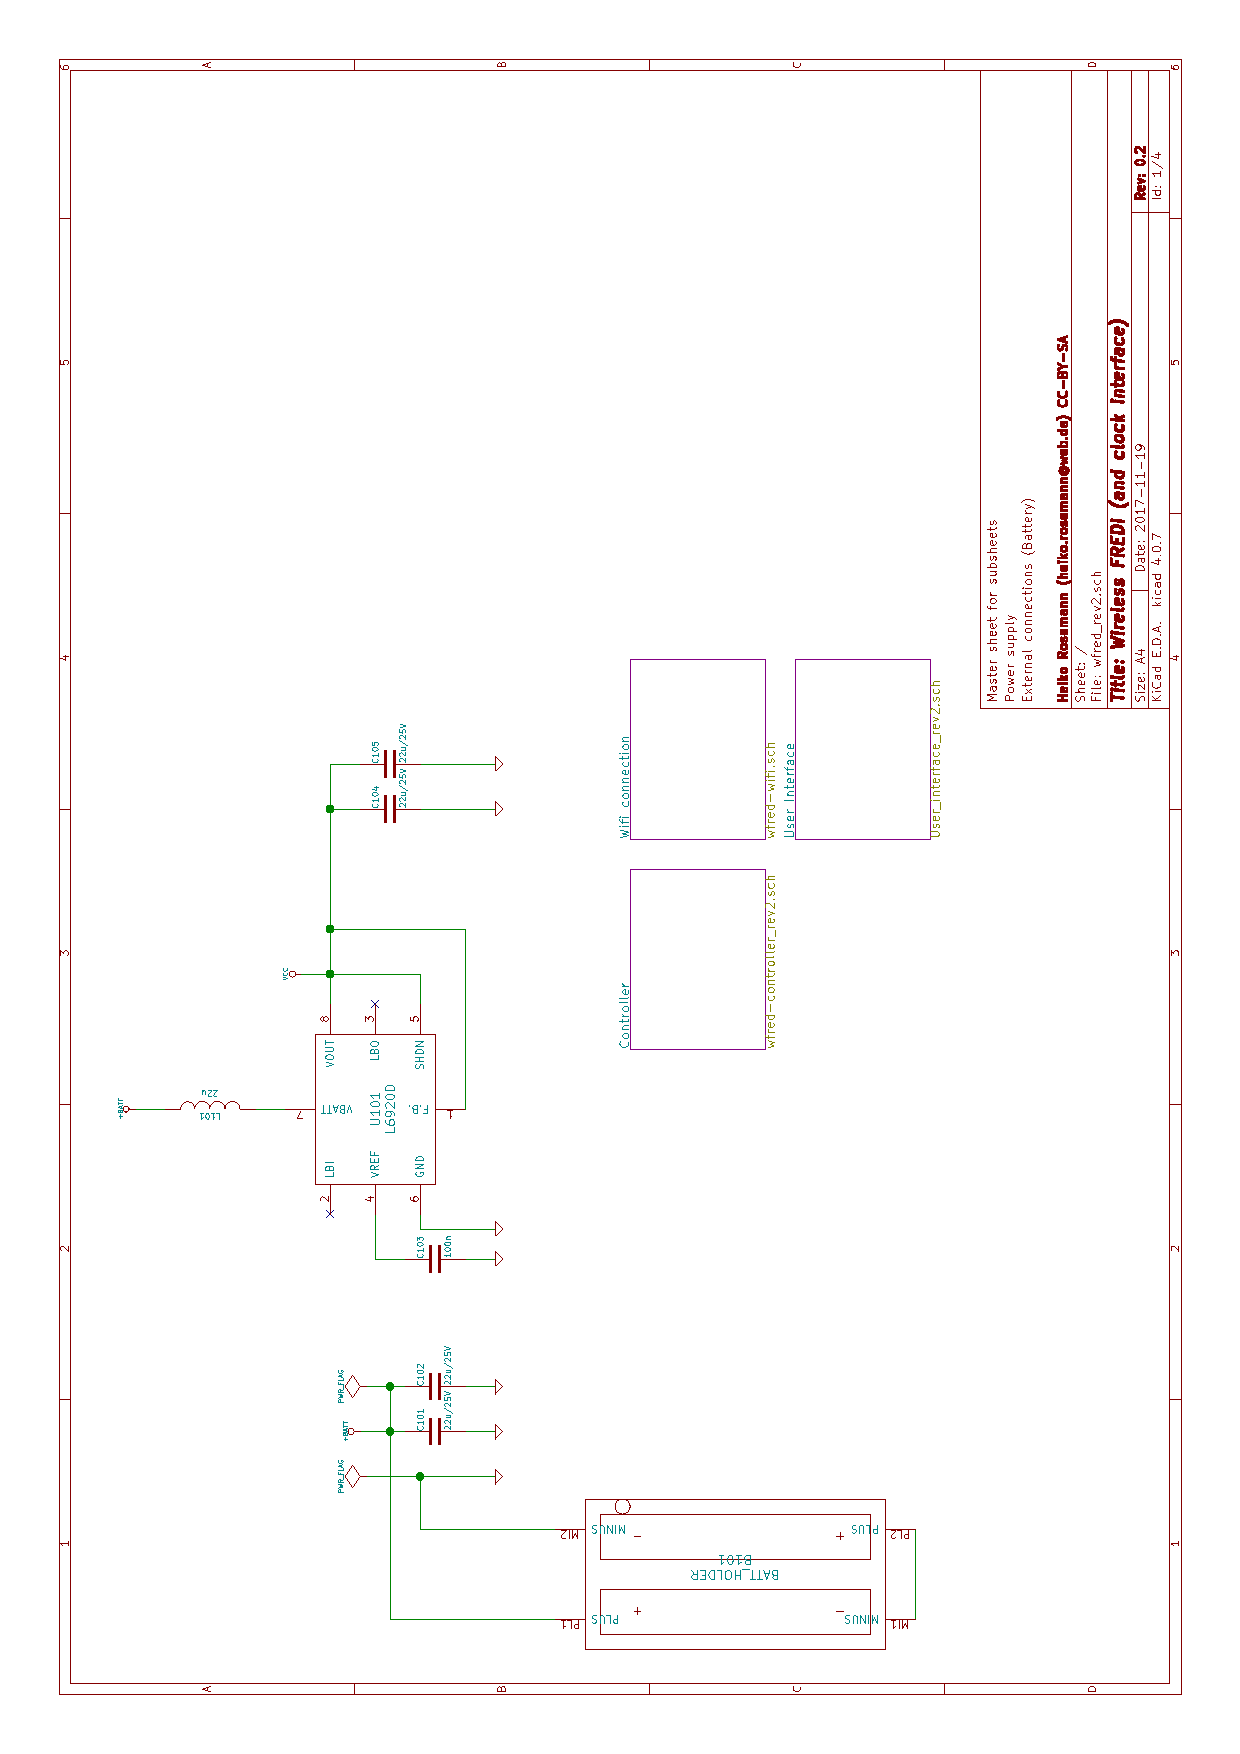
\includegraphics[width=\textwidth]{images/wfred_rev2}
  \caption{Master schematic sheet with batteries and power supply}
  \label{schematicPage1}
\end{figure}

\begin{figure}[tbh]
  \centering
  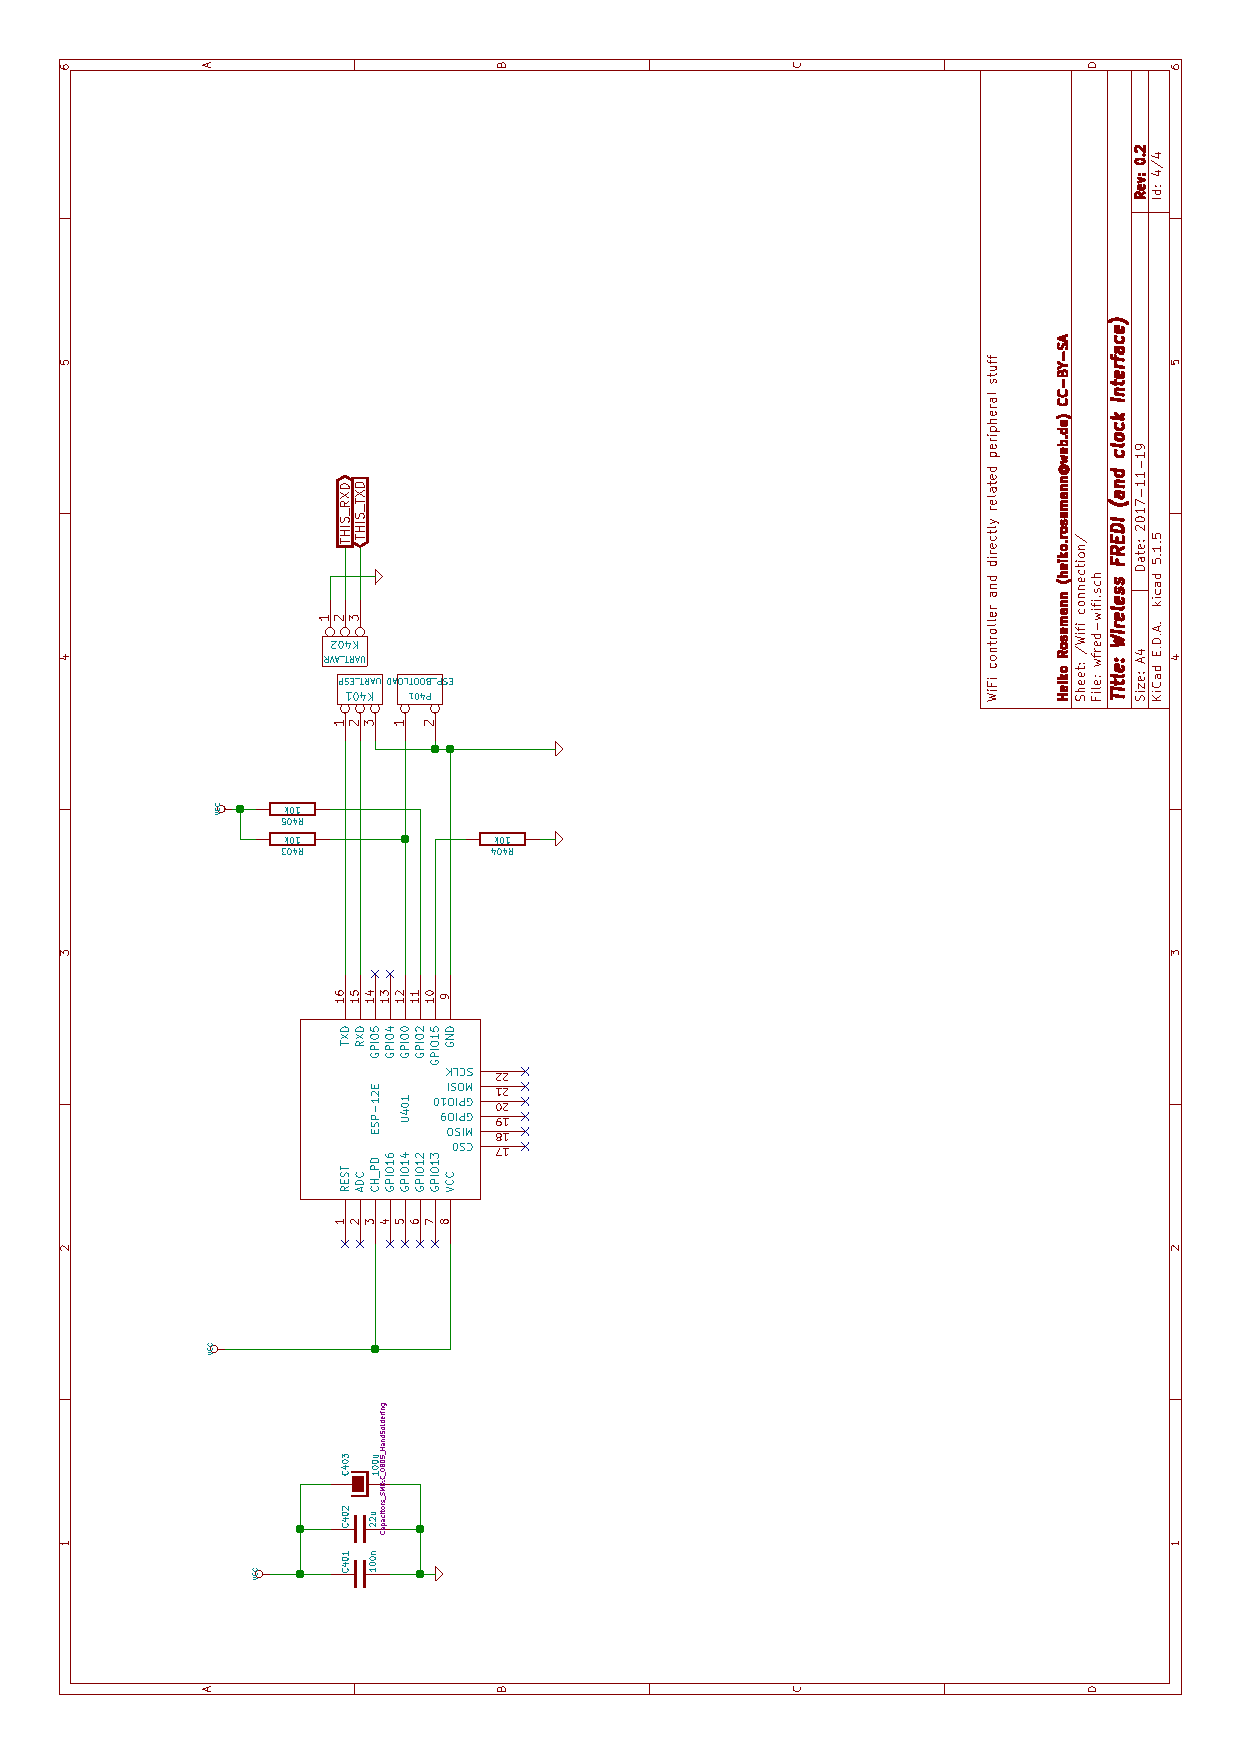
\includegraphics[width=\textwidth]{images/wfred-wifi-Wifi_connection}
  \caption{Schematic sheet including ESP8266 for WiFi connection with bootloader enabling jumper and connection to programming cable}
  \label{schematicPage2}
\end{figure}

\begin{figure}[tbh]
  \centering
  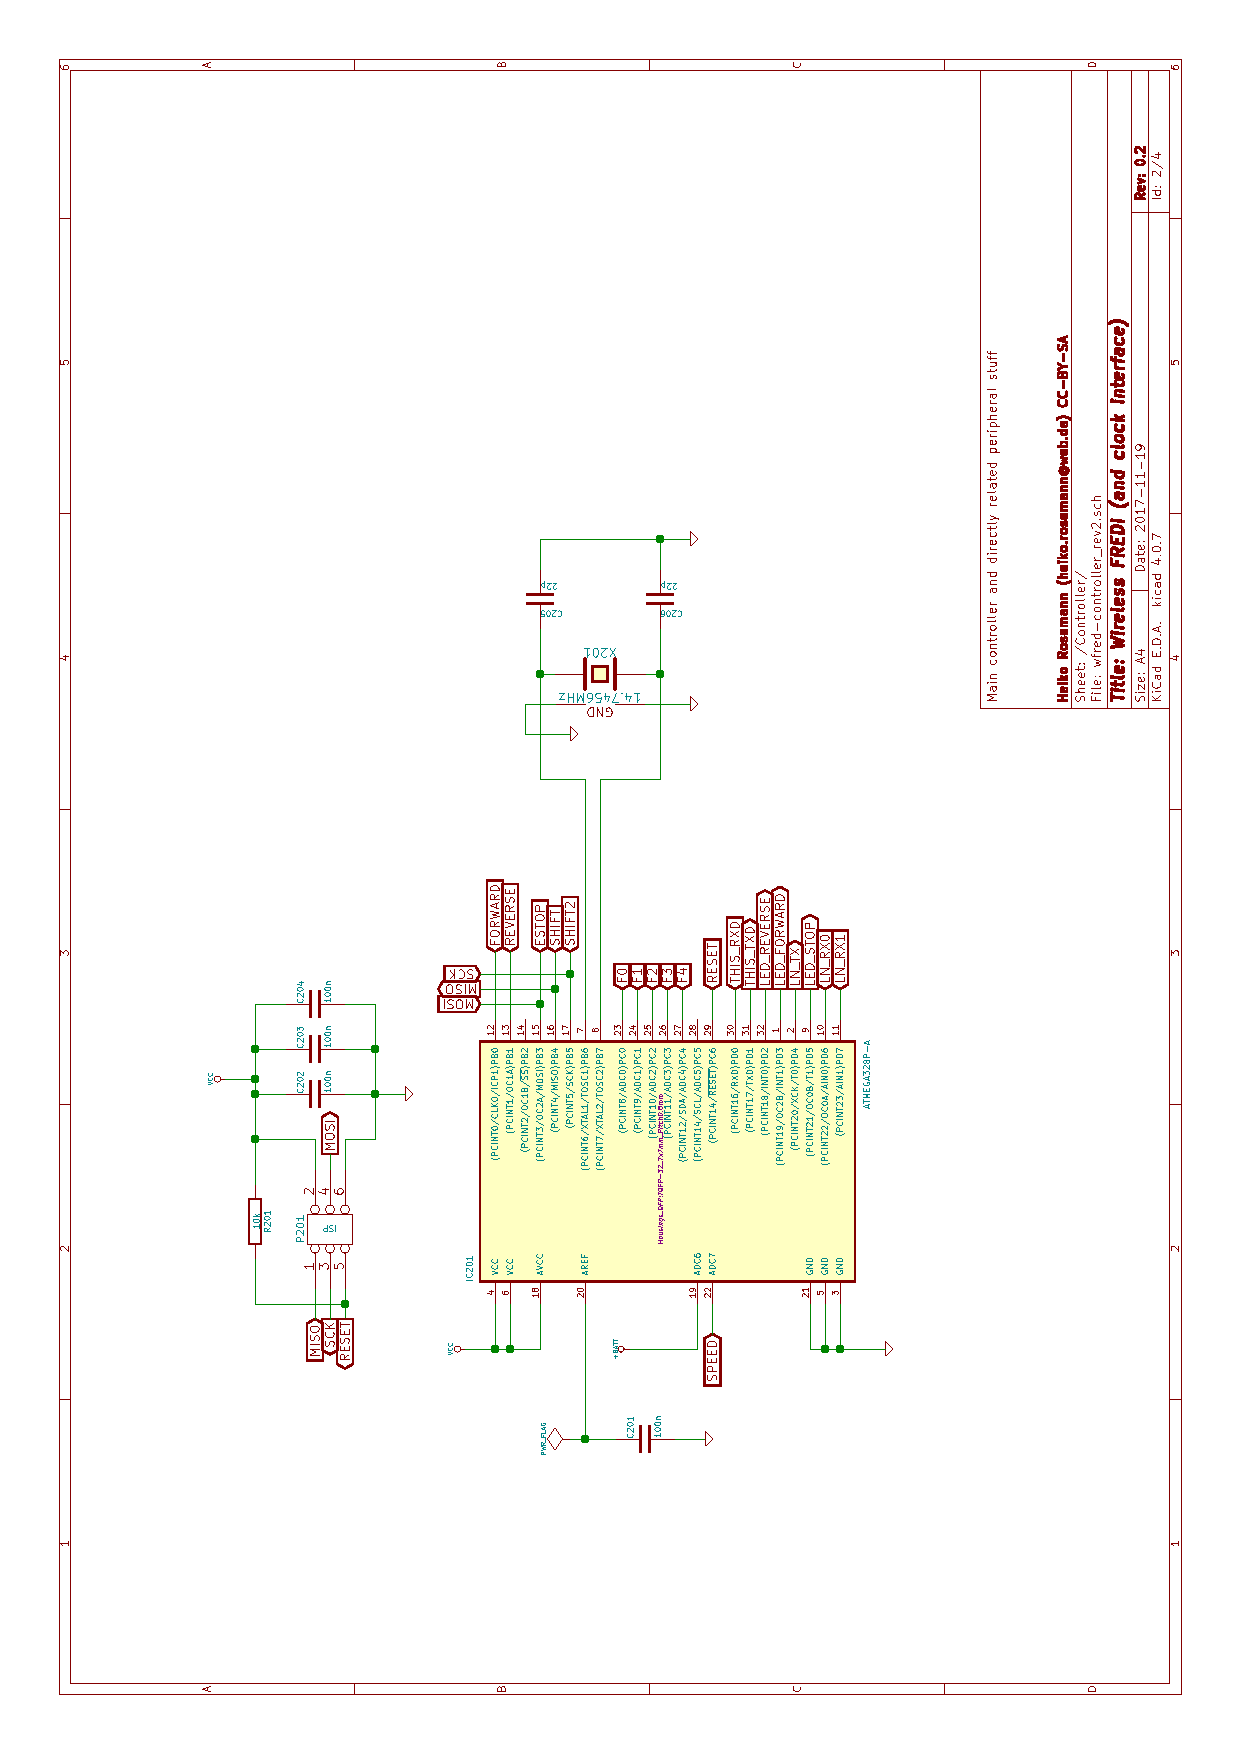
\includegraphics[width=\textwidth]{images/wfred-controller_rev2-Controller}
  \caption{Schematic sheet including ATMega 328P along with crystal and in system programming header}
  \label{schematicPage3}
\end{figure}

\begin{figure}[tbh]
  \centering
  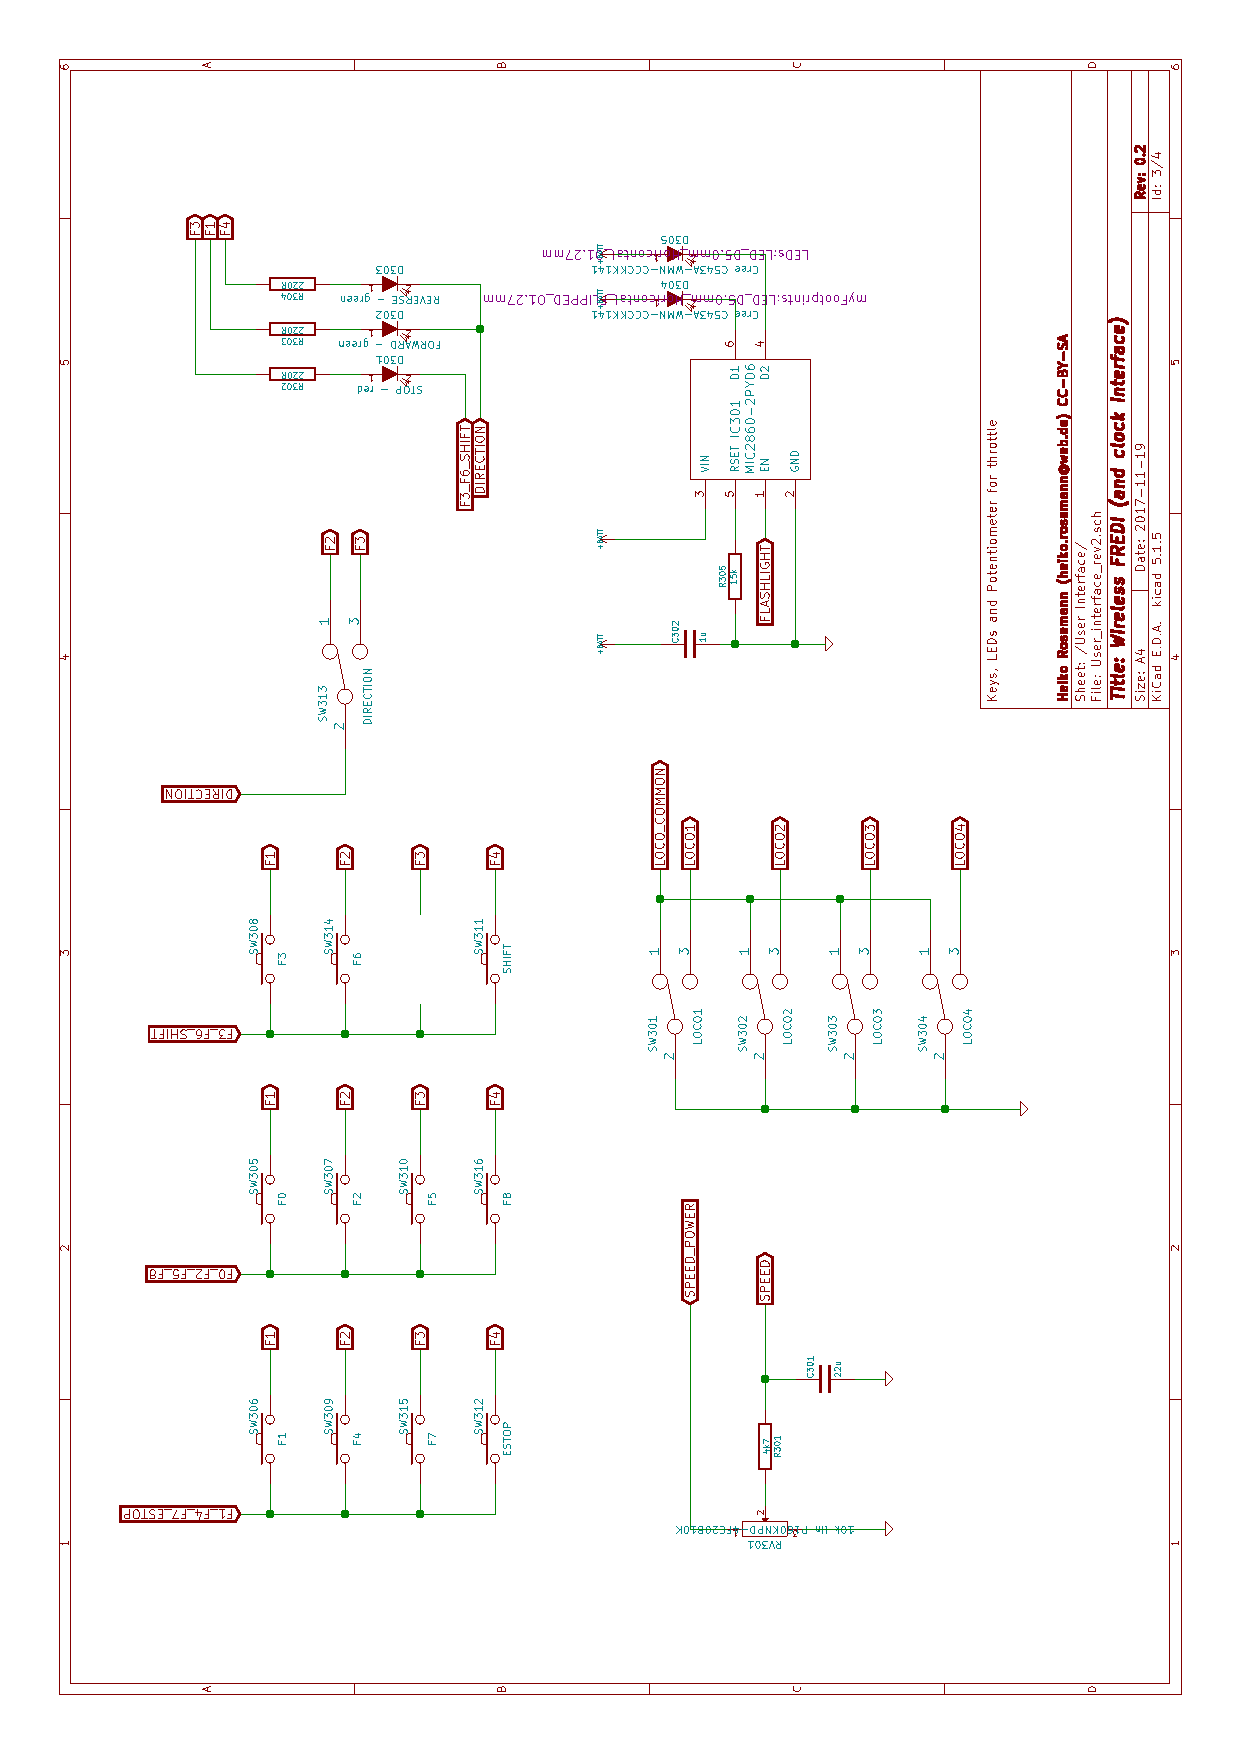
\includegraphics[width=\textwidth]{images/User_interface_rev2-User_Interface}
  \caption{Schematic sheet including pushbutton switches, loco selection switches, direction switch and speed potentiometer}
  \label{schematicPage4}
\end{figure}

\subsection{Hints for building the wiFred}

The PCB has holes in the center of the pushbutton switch footprints and LED footprints to enable transferring their positions to a StrapuBox housing with a sharp needle or similar, and the position of the loco selection switches can also be transferred to the housing by marking it through the non-copper holes at their ends. Figure~\ref{transferHoles} shows the process and it's results. Holes for the pushbutton switches should be drilled at 3.5\,mm diameter and countersunk from the inside. Holes for the LEDs should be drilled at 3\,mm diameter and holes for the speed potentiometer and direction switch at 6.5\,mm or 7\,mm diameter and countersunk. The cutouts for the loco selection switches are best created when the PCB is assembled and carefully cut out with a sharp hobby knife and a file until they fit.

\begin{figure}[tbh]
  \centering
  \includegraphics[width=0.49 \textwidth]{images/_DSC8652}
  \includegraphics[width=0.49 \textwidth]{images/_DSC8653}
  \caption{Using the PCB to transfer the positions of the holes to the housing}
  \label{transferHoles}
\end{figure}

To fit into a StrapuBox 6090 housing, the PCB should be made 0.8\,mm in thickness\footnote{Or less, but then it will more easily bend}. The remaining assembly is a basic exercise in installing all the components to the PCB, listed in table~\ref{wiFredBOM}. From assembling the prototypes, the suggested order of installing the components is as follows:

\begin{table}
  \caption{List of components for the wiFred} \label{wiFredBOM}

  \vspace{0.5em}

  \centering
  \begin{footnotesize}
  \begin{tabular}{|m{5em}|l|l|}
    \hline
    Designator & Package & Designation \\
    \hline
    B101 & KEYSTONE1013 & BATT\_HOLDER \\
    C206,C205 & C\_0805\_HandSoldering & 22p \\
    C301,C105, C104,C102, C101 & C\_0805\_HandSoldering & 22u/25V \\
    C401,C204, C203,C202, C201,C103 & C\_0805\_HandSoldering & 100n \\
    C402 & C\_0805\_HandSoldering & 22u \\
    D301 & LED\_D3.0mm & STOP - red \\
    D302 & LED\_D3.0mm & FORWARD - green \\
    D303 & LED\_D3.0mm & REVERSE - green \\
    IC201 & TQFP-32\_7x7mm\_Pitch0.8mm & ATMEGA328P-A \\
    K401 & Pin\_Header\_Straight\_1x03\_Pitch2.54mm & UART\_ESP \\
    K402 & Pin\_Header\_Straight\_1x03\_Pitch2.54mm & UART\_AVR \\
    L101 & L\_2424\_HandSoldering & 22u \\
    P201 & Pin\_Header\_Straight\_2x03\_Pitch2.54mm\_SMD & ISP \\ 
    P401 & Pin\_Header\_Straight\_1x02\_Pitch2.54mm & ESP\_BOOTLOAD \\
    R301 & C\_0805\_HandSoldering & 4k7 \\
    R304,R303, R302 & C\_0805\_HandSoldering & 470R \\
    R401 & C\_0805\_HandSoldering & 100k \\
    R402 & C\_0805\_HandSoldering & 47k \\
    R405,R404, R403,R201 & C\_0805\_HandSoldering & 10k \\
    RV301 & P160KNPD & 10k lin P160KNPD-4FC20B10K \\
    SW301 & OS102011MS2Q & LOCO1 \\
    SW302 & OS102011MS2Q & LOCO2 \\
    SW303 & OS102011MS2Q & LOCO3 \\
    SW304 & OS102011MS2Q & LOCO4 \\
    SW305 & KSC621G & F0 \\
    SW306 & KSC621G & F1 \\
    SW307 & KSC621G & F2 \\
    SW308 & KSC621G & F3 \\
    SW309 & KSC621G & F4 \\
    SW310 & KSC621G & SHIFT2 \\
    SW311 & KSC621G & SHIFT \\
    SW312 & KSC621G & ESTOP \\
    SW313 & 100SP1T1B1M1QEH & DIRECTION \\
    U101 & TSSOP-8\_4.4x3mm\_Pitch0.65mm & L6920D \\
    U401 & ESP-12E\_SMD & ESP-12E \\
    X201 & Crystal\_SMD\_TXC\_7M-4pin\_3.2x2.5mm\_HandSoldering & 14.7456MHz \\
    \hline
    Housing & StrapuBox 6090 & \\
    & Two Jumpers, 2.54mm & \\
    & Potentiometer Knob & \\
    \hline
  \end{tabular}
  \end{footnotesize}
\end{table}

\begin{enumerate}
\item IC201 and U101 (note: Rotate PCB so Designator is right side up, then Pin 1 is on top left)
\item X201
\item Capacitors and Resistors in 0805 size (only those on the same side as the items before) \label{0805devices}
\item U401
\item LEDs D301 to D303
\item Pushbutton switches SW305 to SW312
\item Loco selection switches SW301 to SW304
\item L101
\item Capacitors and Resistors not installed in step~\ref{0805devices}
\item Pin header P201
\item Pin headers K401, K402 and P401 (correct alignment of K401 and K402 can be assured by adding a jumper before soldering)
\item Direction switch SW313 (screwed into the PCB with an 8\,mm hex nut first, then attached to it's pads using the cutoffs from D301, D302 and D303) and Speed potentiometer RV301 (screwed into the PCB with a 10\,mm hex nut first and slightly shortening the pins before soldering)
\item Battery holder B101
\end{enumerate}

After assembling the PCB with all the components and drilling and cutting the holes and cutouts into the housing, there are few steps left. First, a few protrusions inside the housing need to be removed so the PCB fits properly. Figure~\ref{breakProtrusions} shows how they can be removed easily, remains may be cut off with a hobby knife. Second, new PCB mounting pads need to be installed as shown in figure~\ref{mountingPads}. For the prototype, Forex PVC foam was used, cut with a pair of scissors and glued to the housing with superglue, making sure not to be in the way of any components on the PCB, but any kind of easily worked upon material with a thickness of 3\,mm can be used, as long as it will take self-driving screws (prototype uses 2.9\,mm by 6.5\,mm DIN~7981 screws). Third, the two shift keys need yellow paint on the top and the emergency stop key needs red paint -- either any kind of paint or a paint marker like Edding~751 will do. Finally, both the ESP8266 and the ATMega~328P will need to be programmed as described in the next section.

\begin{figure}[tbh]
  \centering
  \includegraphics[width=0.49 \textwidth]{images/_DSC8654}
  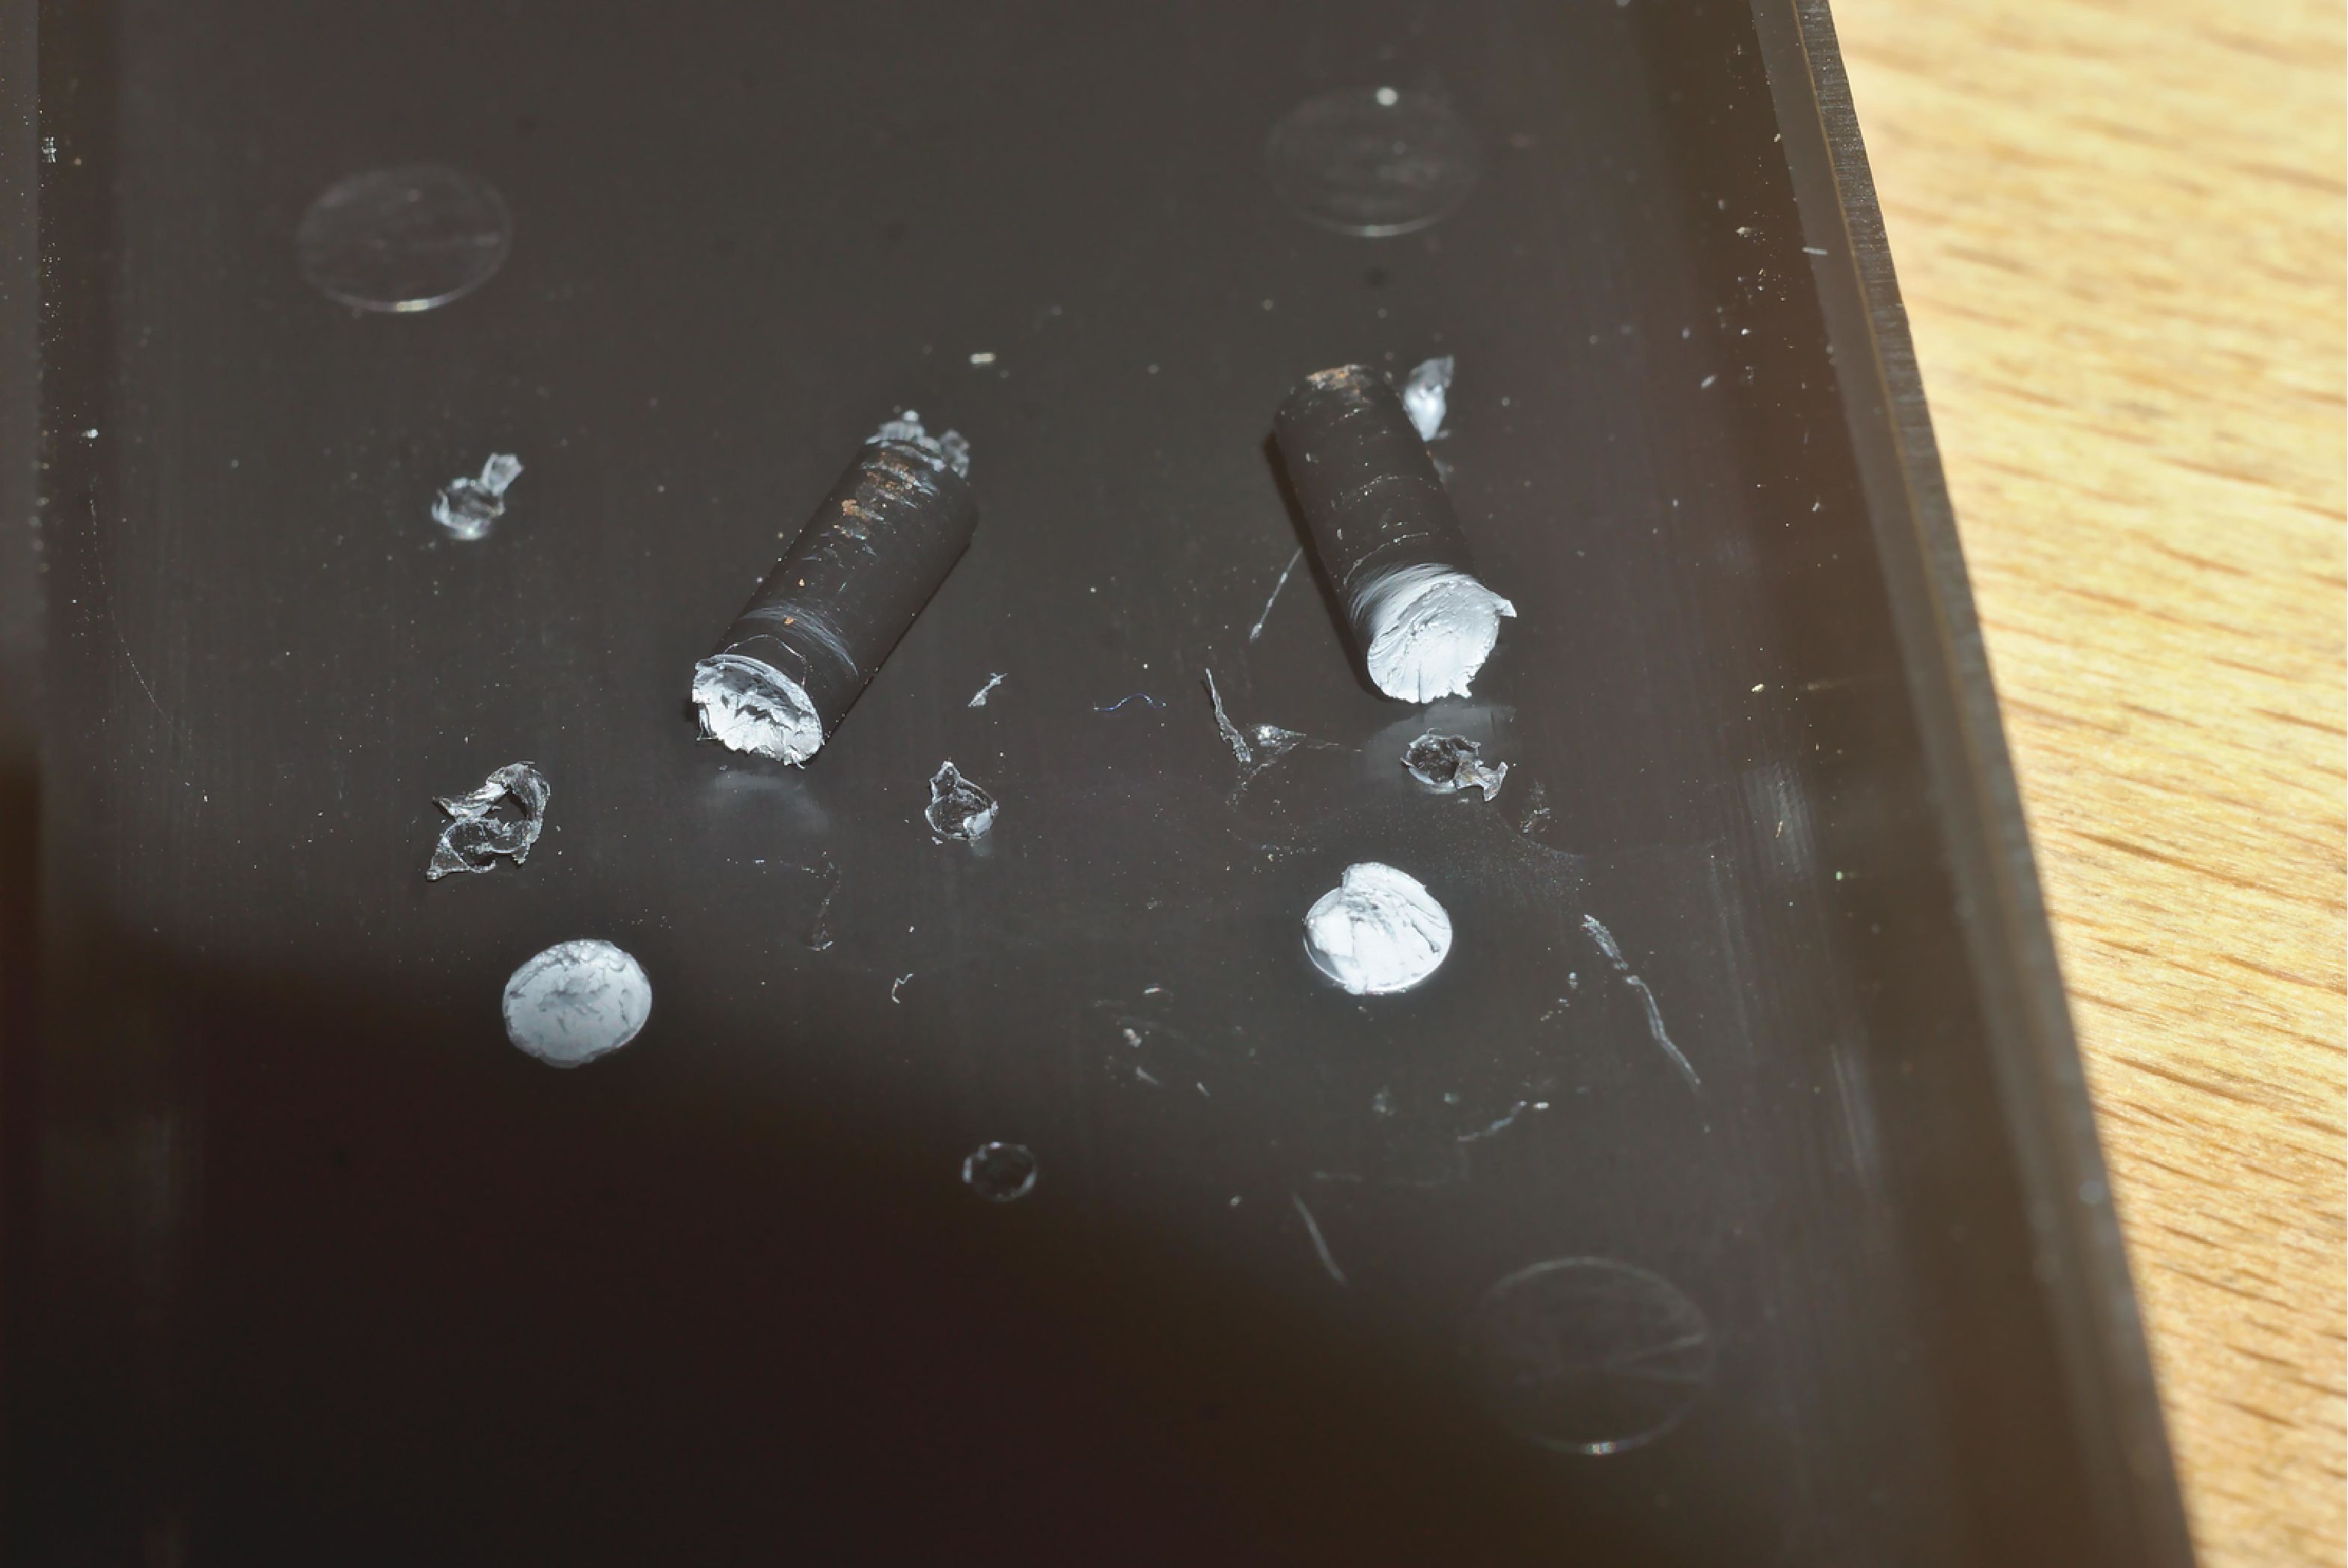
\includegraphics[width=0.49 \textwidth]{images/_DSC8655}
  \caption{Removing protrusions inside the housing so the PCB fits}
  \label{breakProtrusions}
\end{figure}

\begin{figure}[tbh]
  \centering
  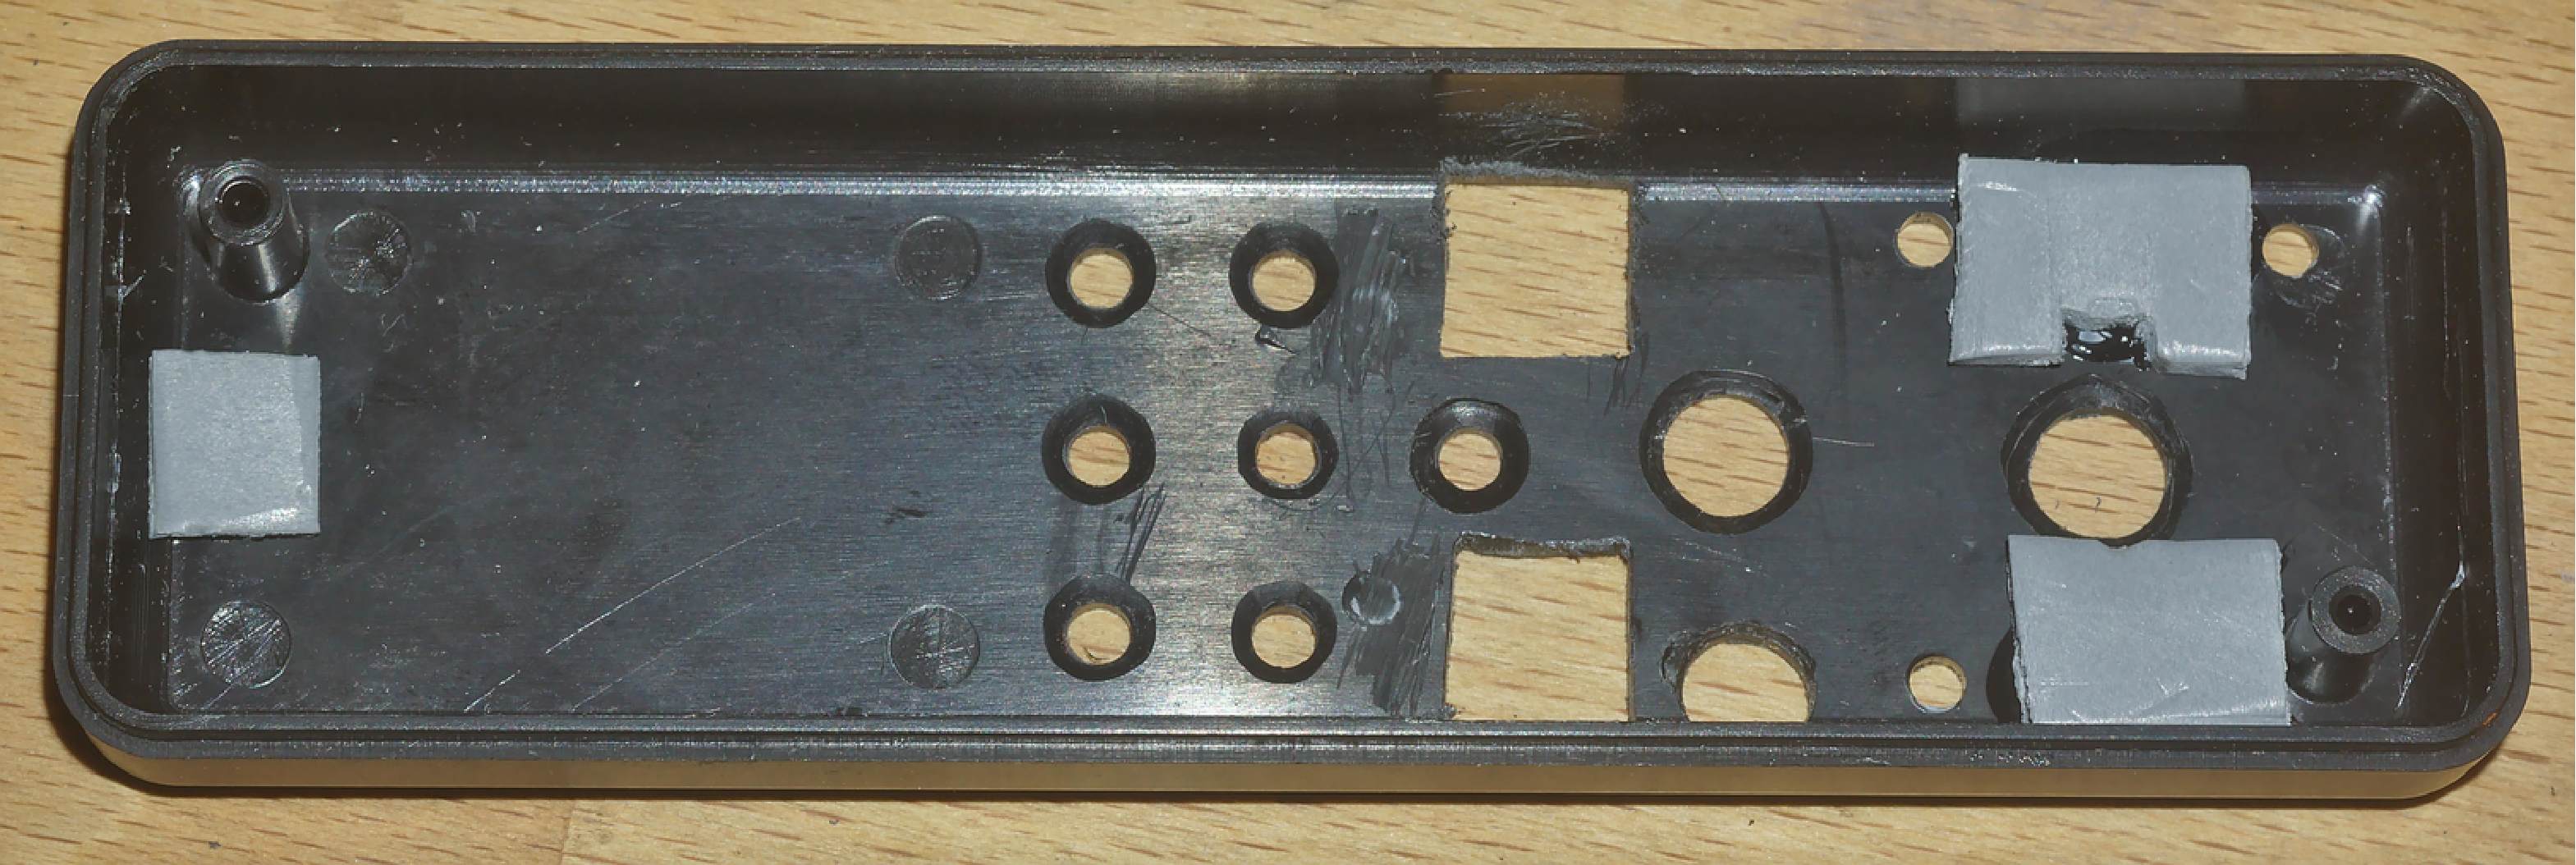
\includegraphics[width=0.8 \textwidth]{images/_DSC8658}
  \caption{New PCB mounting pads made from 3\,mm thick Forex PVC}
  \label{mountingPads}
\end{figure}

\subsection{Programming instructions}

The ESP8266 is programmed using the Arduino IDE connected via a serial or USB-to-serial port to the K401 header as shown in figure~\ref{progESP}. The serial port needs to be at 3.3\,V-levels like from an FTDI232-device run at 3.3\,V.

\begin{figure}[tbh]
  \centering
  \includegraphics[width=0.8 \textwidth]{images/_DSC8637}
  \caption{Programming connection for ESP8266 -- GND on orange wire, then TXD of programming cable (RXD of ESP8266), then RXD of programming cable (TXD of ESP8266)}
  \label{progESP}
\end{figure}

\begin{figure}[tbh]
  \centering
  \includegraphics[width=0.8 \textwidth]{images/_DSC8638}
  \caption{Programming connection for ATMega~328P -- Pin 1 on purple cable}
  \label{progAVR}
\end{figure}

All files in the \textit{software/esp-firmware}-subdirectory of the github repository need to be placed in a folder, then the main sketch \textit{arduino\_main\_sketch.ino.ino} needs to be opened with the Arduino IDE. Settings for the Arduino IDE can be found inside the main file, programming the device should work using the \textit{Upload}-button in the \textit{Sketch}-menu.

To put the ESP8266 into programming mode, a jumper needs to be placed across the P401 header before inserting batteries to start the device in programming mode. The bootloader should show some results on the serial port and during download the LED on the ESP module should flash.

The ATMega~328P is programmed using the regular AVR ISP connection on P201. Pin 1 -- GND -- is towards the PCB edge, as shown in figure~\ref{progAVR}. An ISP dongle with either automatic voltage selection or 3.3\,V supply voltage should be used to avoid placing too high voltage on the ESP, which can only support 3.3\,V power. The firmware for the AVR can be found in the \textit{software/avr-firmware}-subdirectory of the github repository with both a precompiled hexfile and all source code including a Makefile to recompile as needed. After writing the firmware file, also the fuse bits need to be set properly as detailed in the \textit{main.c}-file.

After programming, two jumpers need to be placed between the K401 and K402 pin headers to re-enable communication between the ESP8266 and the AVR.

\section{Wireless clock driver} \label{clock}

\subsection{Usage}

\subsection{Configuration}

For general configuration (WiFi etc.) see section~\ref{throttle_GeneralConf}, as it's the same.

\subsection{Hardware description}

\subsection{Programming instructions}

\section{Options for server setup}

\begin{thebibliography}{99}
\bibitem{jmri}{JMRI: A Java Model Railroad Interface, \textit{http://www.jmri.org}}
\bibitem{jmrihardwaresupport}{JMRI: Hardware Support, \textit{http://www.jmri.org/help/en/html/hardware/index.shtml}}
\bibitem{withrottleApp}{WiThrottle, \textit{http://www.withrottle.com/html/home.html}}
\bibitem{EngineDriver}{Home \textbar\ EngineDriver, \textit{https://enginedriver.mstevetodd.com/}}
\bibitem{fremo}{Home - FREMO - Freundeskreis Europ\"aischer Modelleisenbahner e.V., \textit{https://www.fremo-net.eu/en/home/}}
\bibitem{fred}{Throttle, \textit{http://fremodcc.sourceforge.net/throttle/throttle.en.html}}
\bibitem{uhlenbrock}{Uhlenbrock \textbar\ FRED, der Handregler f\"ur die Intellibox, \textit{https://uhlenbrock.de/de\_DE/produkte/prodarch/I62AD172-001.htm!ArcEntryInfo=0004.41.I62AD172}}
\bibitem{mrc}{Prodigy WiFi, \textit{http://www.modelrectifier.com/Prodigy-WiFi-s/332.htm}}
\bibitem{digitrax}{LocoNet WiFi interface, \textit{http://www.digitrax.com/products/wireless/lnwi/}}
\end{thebibliography}

\begin{versionhistory}
  \vhEntry{0.1}{WIP}{Heiko Rosemann}{Setup first document structure.}
\end{versionhistory}

\end{document}
